\documentclass{beamer}
\usetheme{Madrid}
\usepackage[utf8]{inputenc}  % 可以保留沒關係
\usepackage{xeCJK}
\setCJKmainfont{Noto Sans CJK TC} % 需先測試字型名稱
\usepackage{listings}
\usepackage{xcolor}

\lstdefinelanguage{Lisp}{
  morekeywords={defun, lambda, let, if, cond, car, cdr, cons, list},
  sensitive=true,
  morecomment=[l]{;},
  morestring=[b]"
}

\lstdefinestyle{cppstyle}{
  language=C++,
  basicstyle=\ttfamily\small,
  keywordstyle=\color{blue}\bfseries,
  commentstyle=\color{gray},
  stringstyle=\color{orange},
  numbers=left,
  numberstyle=\tiny\color{gray},
  stepnumber=1,
  numbersep=5pt,
  frame=single,
  breaklines=true,
  showstringspaces=false,
  tabsize=2
}

\lstdefinestyle{lispstyle}{
  language=Lisp,
  basicstyle=\ttfamily\small,
  keywordstyle=\color{purple}\bfseries,
  commentstyle=\color{gray},
  stringstyle=\color{orange},
  numbers=left,
  numberstyle=\tiny\color{gray},
  stepnumber=1,
  numbersep=5pt,
  frame=single,
  breaklines=true,
  showstringspaces=false
}

\begin{document}

\title{資料結構與演算法入門:第 0 章}
\subtitle{資料結構與演算法的簡介}
\author{悠太翼 Yuuta Tsubasa}
\date{\today}

\frame{\titlepage}

\begin{frame}{什麼是資料結構?}
\begin{itemize}
    \item 資料結構是「用來儲存與組織資料的方式」
    \item 常見資料結構:
    \begin{itemize}
        \item 陣列 Array:可以儲存一堆有序的資料
    \end{itemize}
\end{itemize}
\begin{center}
    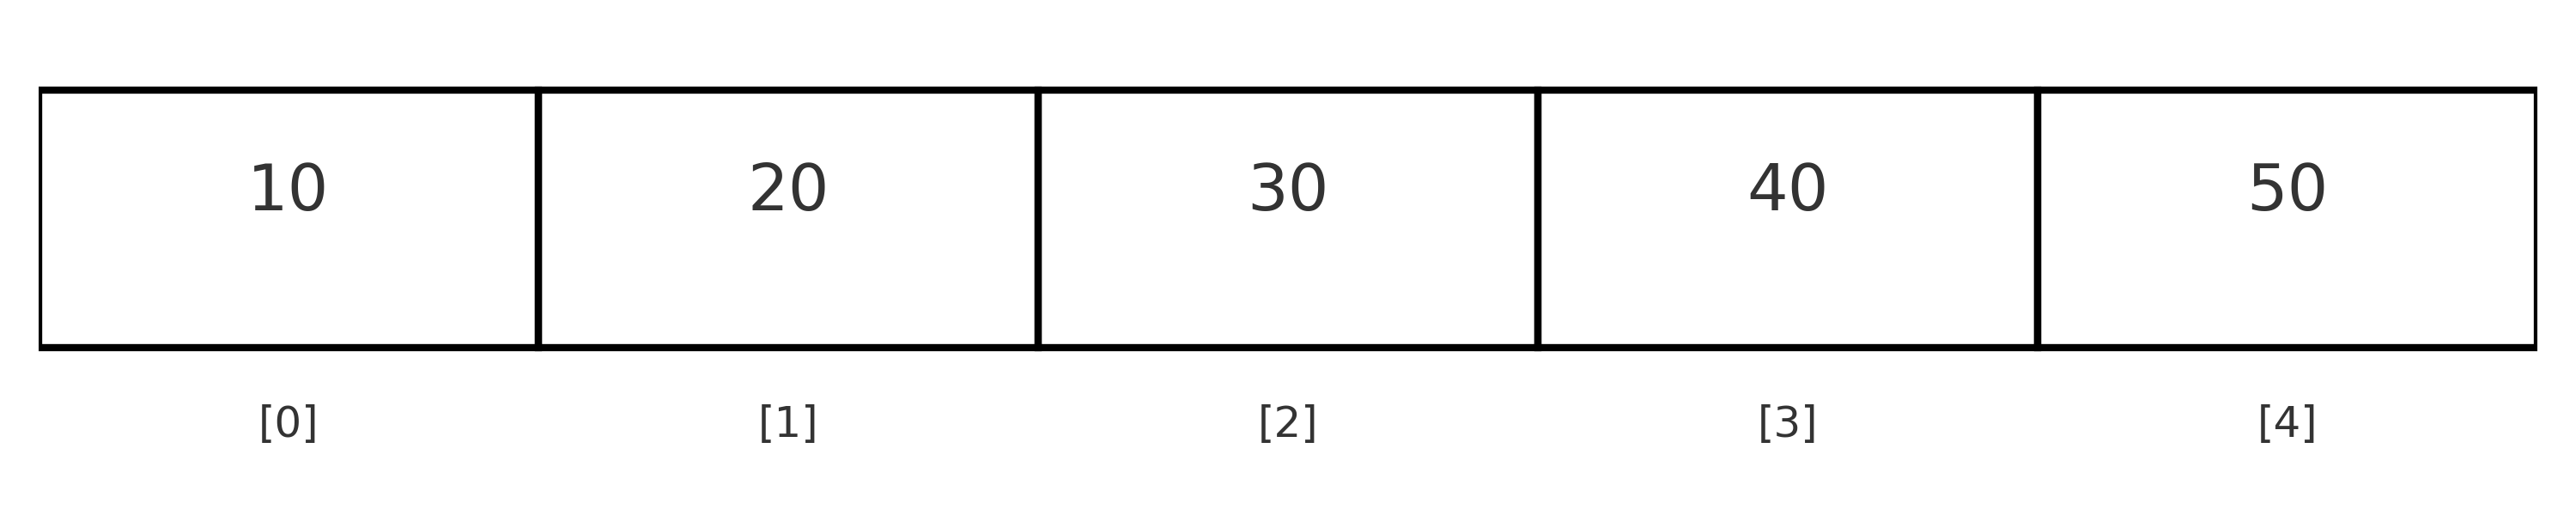
\includegraphics[width=0.8\textwidth]{images/array_example.png}
\end{center}
\end{frame}

\begin{frame}{什麼是演算法?}
\begin{itemize}
    \item 一組解決問題的步驟或流程
    \item 演算法處理輸入資料,產生正確輸出
    \item 範例:
    \begin{itemize}
        \item 排序學生成績:使用排序演算法(Sort)
    \end{itemize}
\end{itemize}
\begin{center}
    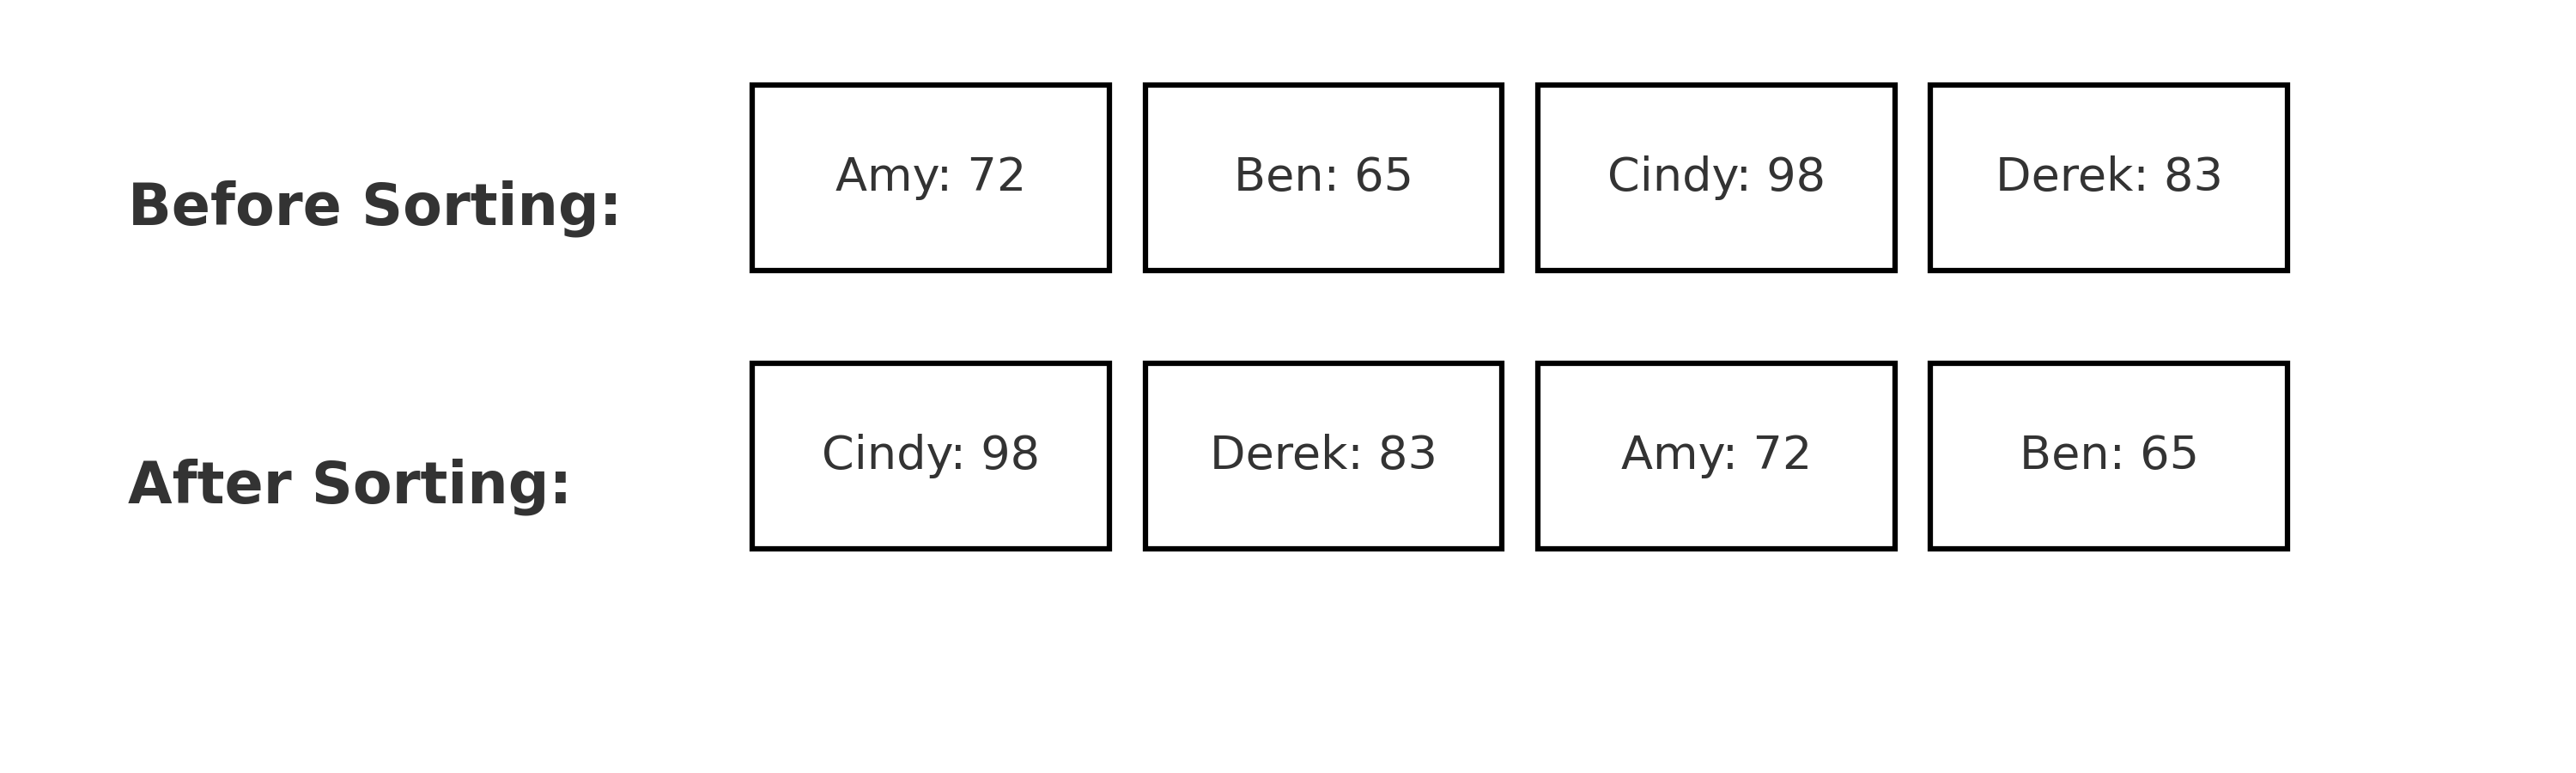
\includegraphics[width=0.8\textwidth]{images/sort_example_students.png}
\end{center}
\end{frame}

\begin{frame}{什麼是演算法?(乘法的例子)}
\begin{itemize}
    \item 假設我們要計算 \texttt{a × b},其中 \texttt{a = 12},\texttt{b = 5}
    \item 可以怎麼做呢?
\end{itemize}

\vspace{1em}
\begin{block}{文字描述}
我們可以從日常語言出發,這樣說明:
\begin{itemize}
    \item 從 0 開始
    \item 把 12 加上 5 次
    \item 得到的結果就是答案
\end{itemize}
\end{block}

\vspace{0.5em}
\begin{itemize}
    \item 接下來,讓我們轉換成「演算法虛擬碼」的形式!
\end{itemize}
\end{frame}

\begin{frame}{乘法的演算法(虛擬碼)}
\begin{block}{虛擬碼(Pseudo Code)}
\begin{enumerate}
    \item 設定 result = 0
    \item 重複執行 b 次:
    \begin{itemize}
        \item 每次把 a 加到 result 裡
    \end{itemize}
    \item 回傳 result
\end{enumerate}
\end{block}

\vspace{1em}
\begin{itemize}
    \item 虛擬碼就是「不寫死語言」的演算法表達方式
    \item 我們可以將它轉換成 C++、Python …等實際語言
\end{itemize}
\end{frame}

\begin{frame}[fragile]{程式碼示範:C++ 實作}
\vspace{-0.5em}
\begin{lstlisting}[style=cppstyle]
int multiply(int a, int b) {
    int result = 0;
    for (int i = 0; i < b; i++) {
        result += a;
    }
    return result;
}

int result = multiply(12, 5);
\end{lstlisting}
\end{frame}

\begin{frame}[fragile]{進階補充:LISP 程式碼範例(可略過)}
\begin{itemize}
    \item 以下是用 LISP 撰寫的乘法演算法(用遞迴加法實作):
\end{itemize}

\vspace{0.5em}
\begin{lstlisting}[style=lispstyle]
(defun multiply (a b)
  (if (= b 0)
      0
      (+ a (multiply a (- b 1)))))

(print (multiply 12 5))
\end{lstlisting}

\vspace{1em}
\begin{block}{數學上的遞迴定義}
\[
a \times b =
\begin{cases}
0 & \text{如果 } b = 0 \\
a + (a \times (b - 1)) & \text{如果 } b > 0
\end{cases}
\]
\end{block}
\end{frame}

\begin{frame}{為什麼要學資料結構與演算法?}
\begin{itemize}
    \item 提升解決問題與邏輯思考能力
    \item 寫出效能高、維護性好的程式
\end{itemize}

\vspace{1em}
\begin{center}
    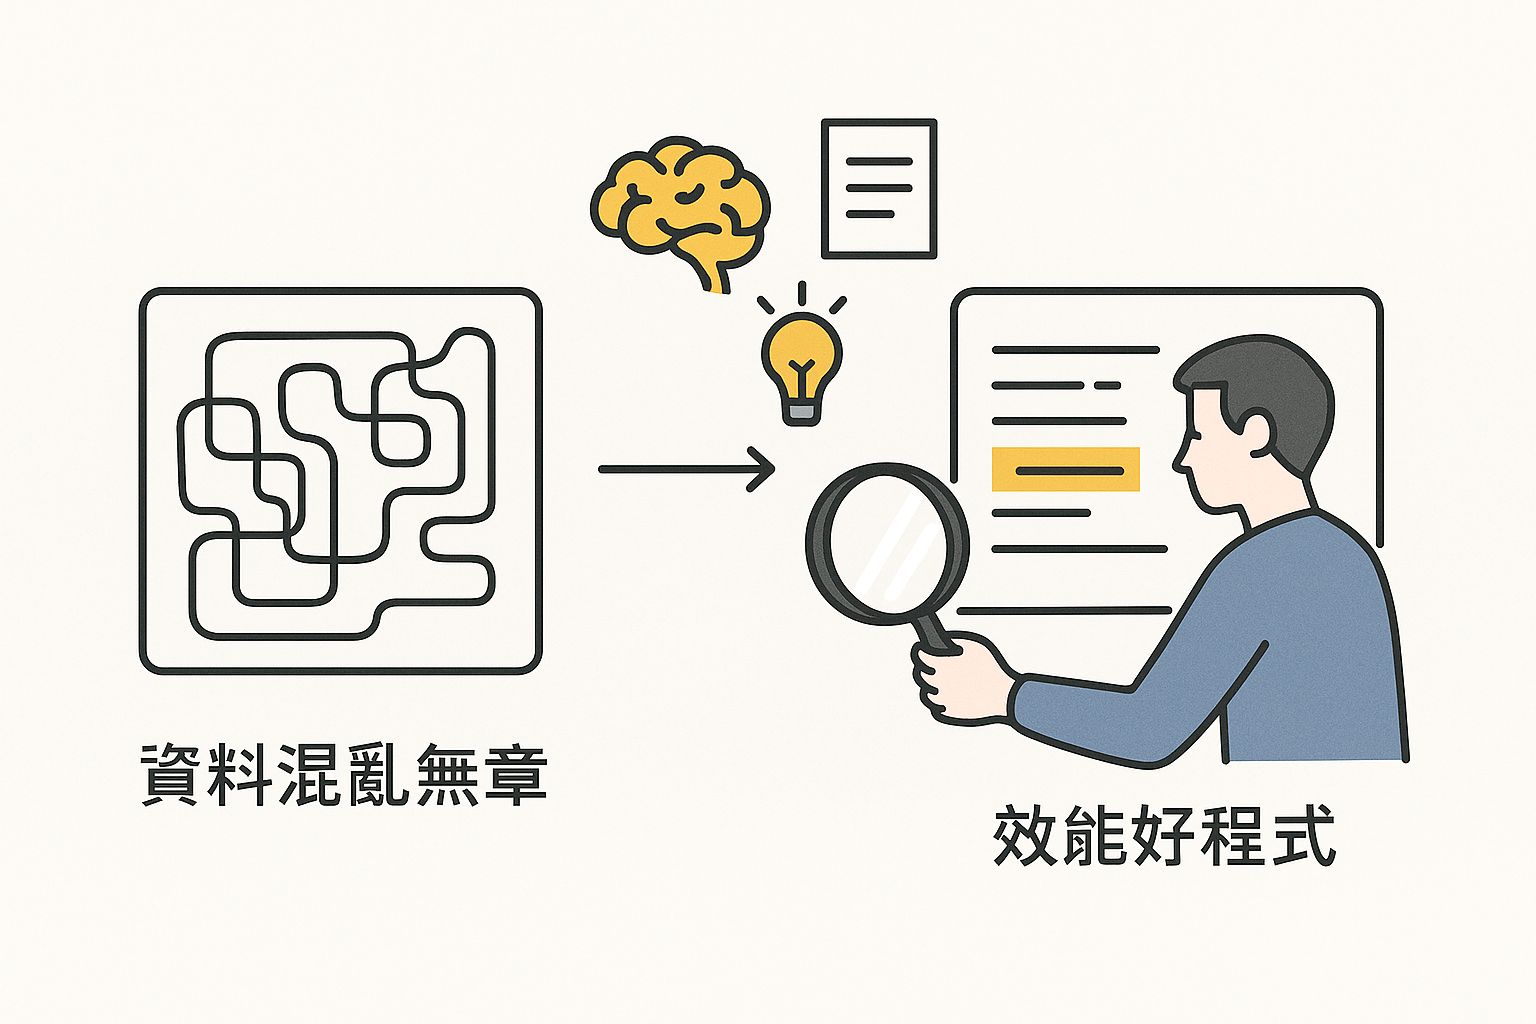
\includegraphics[width=0.6\textwidth]{images/why.png}
    
    {\tiny 圖片來源:ChatGPT}
\end{center}
\end{frame}

\begin{frame}{課程開始!}
\begin{itemize}
    \item 接下來我們會從「演算法複雜度分析」開始學習!
    \item 看懂 O(n)、O(n²) 這些符號到底代表什麼意思~
    \item Ready?那就進入第一章吧!
\end{itemize}

\vspace{1em}
\begin{center}
    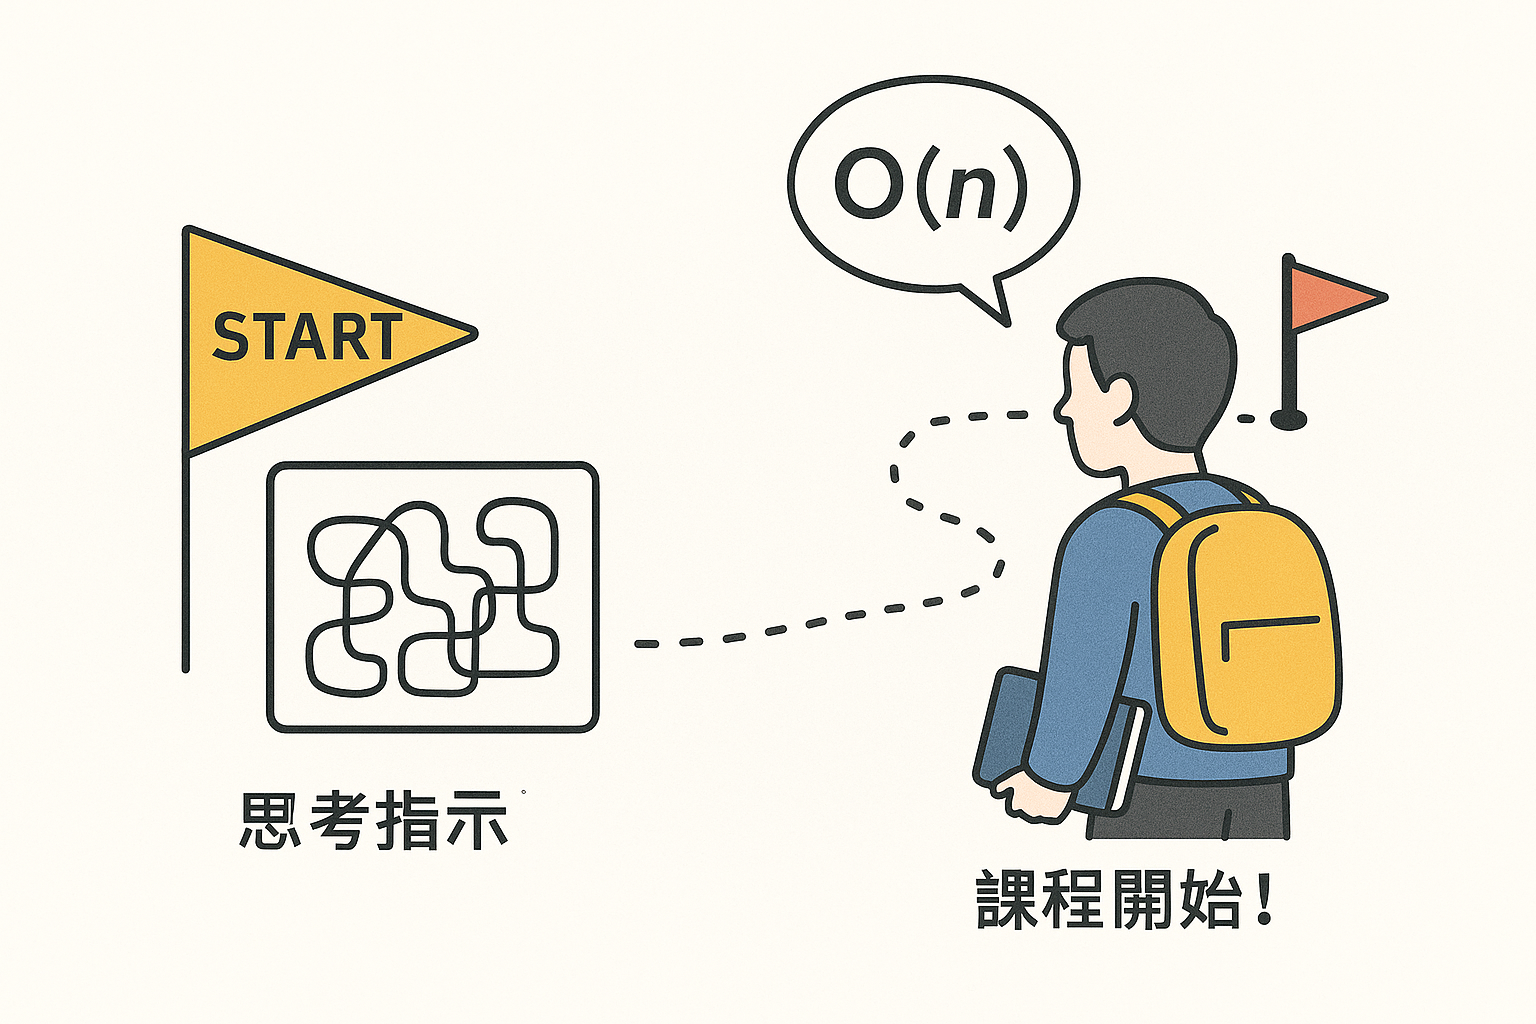
\includegraphics[width=0.6\textwidth]{images/next.png}
    
    {\tiny 圖片來源:ChatGPT}
\end{center}
\end{frame}

\end{document}
